% !TeX root = ../../book.tex
\section{重审-重做-重生}\label{sec:section1.3}

到目前为止,我们一直试图从逻辑的角度激发和解释数学推理和证明撰写,但在此过程中,我们使用了一些你可能熟悉或不熟悉的数学概念和技术。当然,在研究数学时,逻辑和理性思考很重要,但这只是冰山一角。我们试图解释如何组织数学思想,并以一种有意义的方式构建它们,使其他人相信某个特定的事实,但这些思想必须包含与该事实相关的数学概念!

例如,如果没有对几何学的基本了解:三角形是什么,三角形、直线和角度的一些基本性质等等,我们就不可能看到毕达哥拉斯定理的任何证明。我们还假设读者理解什么?许多步骤都涉及算术,例如通过乘以相同因子或减去两个方程来处理多个方程,等等。这些想法现在可能是你的第二天性,但在某个时候你一定学习过这些东西,并了解它们为何以及如何实际发生作用,以便你将来可以安全且恰当地使用它们。

回顾一下前面几节中的证明。我们都用了什么数学思想?试着写下来,并思考你是何时以及如何了解它们的。尝试写下一些我们可能在没有明确说明的情况下使用的具体事实,并思考为什么我们要这样做。另外,试着找到一些我们提出主张但不一定完全解释为什么它一定\textbf{为真}的例子。例如,在毕达哥拉斯定理的 ``证明 1'' 中,我们在一个正方形内画了四个相同的三角形,然后说里面的图形也是一个正方形。这是\text{真}的吗?我们怎么能这么确定呢?尝试证明一下!

\subsubsection*{先验知识}

要点是,巧妇难为无米之炊,如果不注入一些有意义的数学内容,我们实际上就无法撰写证明。因此,本书的主要目标之一是与你分享一些有趣的数学事实。有时,这涉及使用你已经了解和以前见过的对象(例如三角形或质数)并尝试用它们做新的事情。有时,我们会向你介绍全新的数学对象(例如等价关系或二项式系数)并使用它们。现在,我们想做的是讨论一些我们将经常使用的数学对象和概念,这些对象和概念你可能以前见过。但我们不假设所有这些对象和概念你都见过,这些思想快速学习/重新学习起来都不太难,并且它们在本书的剩余部分以及你数学生涯的剩余部分非常有用!本节中和本节最后提供了一些问题供你解决,以便为你提供一些练习。

\subsection{速算}

我们不期望你心算六位数乘法或类似的事情,但是能够通过加法、减法和乘法来运算``小''数字是一项重要的技能。当然,计算器和计算机程序可能会有所帮助,但我们希望每当我们需要添加几个四位数字时,没有必要运行在 \verb|Maple| 或 \verb|Mathematica| 或 \verb|TI-89| 上。技术在准确性和时间效率上为我们提供了许多便利,但当我们过于依赖这些设备时,我们就会削弱验证自己答案的能力(例如,在出现拼写错误或敲错按键的情况下),并且当我们过于频繁地使用它们时,我们可能根本无法节省任何时间!

我们鼓励你不断尝试在脑海中或在一张草稿纸上执行遇到的任何算术步骤。任何问题/谜题都很少涉及``大''数字的计算,即使有,也可能有一种特殊的技巧可以将问题简化为更容易的问题。例如,尝试解决以下一系列问题,看看你注意到了什么。

\begin{problem}
    对于以下每个乘式,判定结果数字的最后一位。如果您的答案是``零'',则尝试确定结果数字末尾包含\emph{多少个}零。
    \begin{enumerate}
        \item $1 \cdot 2 \cdot 3 \cdot 4 \cdot 5$
        \item $1 \cdot 2 \cdot 3 \cdot \dots \cdot 10$
        \item $1 \cdot 2 \cdot 3 \cdot \dots \cdot 25$
        \item $1 \cdot 2 \cdot 3 \cdot \dots \cdot 100$
        \item $1 \cdot 2 \cdot 3 \cdot \dots \cdot 1000$
        \item $1 \cdot 2 \cdot 3 \cdot \dots \cdot 10000$
        \item $1 \cdot 2 \cdot 3 \cdot \dots \cdot 10^9$
    \end{enumerate}
    尝试写几句话来向朋友解释你上面使用的过程。也就是说,给定任意数字 $n$,请解释如何判定 $1\cdot2\cdot3\cdot \dots \cdot n$ 相乘所得数字末尾零的个数。
\end{problem}

你注意到了什么?前几次你用过计算器吗?这当然可行,或者你甚至可以手工完成前两到三个,但这对你后面的计算有何帮助?这对你解释你的过程有何帮助?当然,你需要找到一种更通用的方法来解决这个问题,在某些情况下,使用计算器或计算机可能会对你有所帮助,但它不会为你提供任何对答案的洞察。\\
如果你还没有弄清楚一般过程,给你一点小提示:
\begin{hint}
    想想乘法运算中出现了多少 $2$ 的倍数和 $5$ 的倍数。试着把它们配对。(为什么要这么做?)
\end{hint}

\subsection{代数魔咒}

\subsubsection*{解线性方程组}

线性方程组只是一组方程,这些方程涉及一定数量的变量(均为一次方,因此是线性的)乘以系数并相加,然后设置为等于一些常数。系数和常数满足特定的条件,可以确保是否有解(事实上,是否存在无限多个解或只有一个解),但我们不会讨论这些特定的细节。可以说,我们在本书中要处理的方程组将具有唯一解,这意味着我们拥有的方程数量将与所涉及的变量数量相同。提前知道这一点的前提下,我们如何操作方程组来找到唯一解?

在实践中,求解方程组最快的方法取决于系数和常数,也许还取决于如何应用我们将要介绍的方法。也就是说,简单地遵循这些方法总是会在短时间内奏效,所以在任何给定的情况下都不要太在意找到绝对最快的方法。

\begin{method}{方法 1: }
    第一种方法涉及两个方程组和两个未知数。这种情况下,我们可以使用其中一个方程来表示一个变量,然后将其代入第二个方程,得到只有一个未知数的方程。由此,我们可以找到一个变量的值,并将其代入另一个方程可以得到另一个变量的值,从而获得我们想要的解。让我们用一个特定的例子来看看这个过程的实际操作。考虑以下方程组:
    $$
    \begin{cases}
        \enspace\: 7x+4y =-2 \\
        -2x+3y =13
    \end{cases}
    $$
    按照我们刚刚描述的方法,我们将整理第一个方程,将 $y$ 写成 $x$ 的形式
    \[y = \frac{1}{4}(-2-7x)\]
    然后将其代入第二个方程
    \[-2x + 3 \cdot \frac{1}{4}(-2 - 7x) = 13\]
    并求解关于 $x$ 的新方程:
    \begin{align*}
        -2x-\frac{3}{2}-\frac{21}{4}x &= 13 \\
        -\frac{29}{4}x &= \frac{29}{2} \\
        x &= -2
    \end{align*}
    然后,我们将在 $x$ 的值代入到第一个方程,求解 $y$: 
    \begin{align*}
        7 \cdot (-2) + 4y &= -2 \\
        4y &= -2+14 = 12 \\
        y &= 3
    \end{align*}
    因此,求得解为 $(x, y) = (-2, 3)$。
\end{method}

如果我们用第二个方程而不是第一个方程得到的 $x$ 值会怎样? 结果也会得到相同的 $y$ 值,只是也许计算上会稍微快一些。或者,如果我们反过来,用 $y$ 表示 $x$,求解 $y$,然后代入再求解 $x$,会怎么样?同样,我们会得到相同的解,但也许数会更``好''算,并为我们节省几秒钟的时间。这就是我们所说的不用担心找到最``有效''的方法的意思。当然,有多种方法可以求解这个方程组,但它们最终源于相同的方法(代入和求解),并产生相同的解。

\begin{method}{方法 2: }
    求解由两个方程和两个未知数组成的方程组的另一种方法是将两个方程乘以特定的值,然后将它们相加,适当地选择这些乘法器,从而消除其中一个变量。使用上面的例子,我们可以将第一个方程乘以 $2$,将第二个方程乘以 $7$,使两个方程中 $x$ 的系数相等但相反;然后,将方程相加,将系统简化为一个仅包含未知数 $y$ 的方程。步骤如下:
    \begin{align*}
        2 \cdot (7x+4y &= -2) \\ 
        7 \cdot (-2x+3y &=13) \\
        14x + (-14x) + 8y + 21y &= -4 + 91 \\
        29y &= 87 \\
        y &= 3
    \end{align*}
    然后,我们可以将该值代入第一个或第二个方程,并求解 $x$。
\end{method}

你可以使用这两种方法中的任何一种来求解任何由两个方程和两个未知数组成的方程组。根据所涉及的数字,也许其中一个会比另一个快一点,但无论哪种方式,都不会节省超过一分钟的时间,因此只要选择其中之一就好。

\begin{method}{方法 3: }
    有时以图形方式解释这些方程组会很方便;这通常不是识别方程组特定解的有效方法,但它可以指示解是否存在,并粗略估计解的大小。

    对于两个未知数,我们可以通整理将诸如 $ax+by=c$ 形式的方程解释为平面中的一条直线:$y = -\frac{a}{b}x+\frac{c}{b}$。这条直线斜率为 $-\frac{a}{b}$, $y$ 轴截距为 $\frac{c}{b}$。给定两个这样的方程,我们可以在平面上画出两条线,并直观地找到交点。该点的 $(x, y)$ 坐标正是我们通过求解上述方程组找到的解。

    \begin{center}
        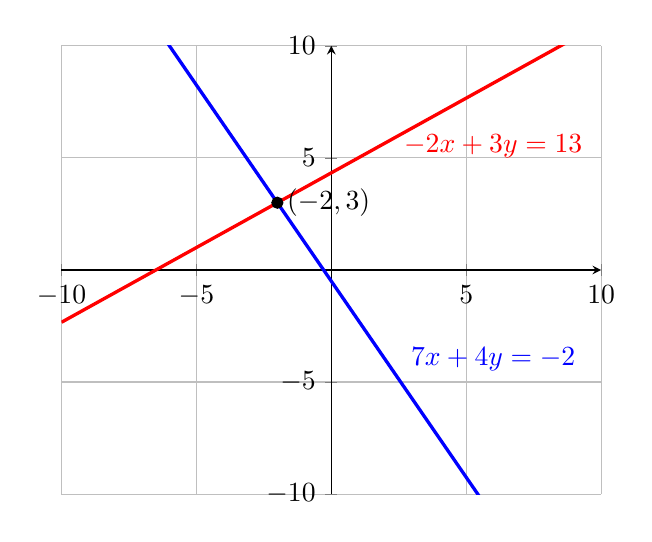
\begin{tikzpicture}
            \begin{axis}[
                axis lines=middle,
                grid=both,
                grid,
                ymin=-10,
                ymax=10,
                xmin=-10, 
                xmax=10
                ]       
                \addplot[mark=none, blue, very thick] coordinates {(-10,17) (10,-18)} node[above] at (axis cs:6,-5) {$7x+4y=-2$};
                \addplot[mark=none, red, very thick] coordinates {(-10,-2.3333) (10,11)} node[below] at (axis cs:6,6.5) {$-2x+3y=13$};
                \addplot[mark=*] coordinates {(-2,3)} node[right] at (axis cs:-2,3) {$(-2,3)$};
            \end{axis}
        \end{tikzpicture}
    \end{center}

    这种可视化方法也适用于三个方程和三个未知数的方程组,但这需要在三维空间中绘制图线。这在实践中可能很难做到,但在技术上是可行的。同样的概念也适用于多个方程和多个未知数,但在四维或更高维上画``线''对我们人类来说是可能是无法想象的!
\end{method}

\begin{method}{多于两个变量:消元!}
    该方法的下一部分建立在第一部分的基础上,通过不断应用第一部分的方法,将两个以上方程(和未知数)的方程组简化为更小的方程组,最终得到两个方程和两个未知数的方程组。我们通过一个三个方程和三个未知数的方程组来说明该方法,如下所示:
    $$
    \begin{cases}
        \enspace\: 6x - 3y + \enspace z = -1 \\
        -3x + 4y - 2z = 12 \\
        \enspace\: 5x + \enspace y + 8z = 6
    \end{cases}
    $$
    第一个目标是消除三个变量中的一个。本质上,这可以通过两种方式之一来完成,就像两个方程和两个未知数的方法一样。假设我们要从方程组中消除 $z$;我们可以尝试以某种方式用 $x$ 和 $y$ 来表示 $z$ 并代入,或者我们可以将某些方程乘以系数并相加,从而消除 $z$。这里唯一的区别是,无论我们选择哪种方法,我们都需要执行两次。我们用第一个方程得到
    \[z = -6x + 3y - 1\]
    将 $z$ 的表达式代入第二个和第三个方程后,我们将得到一个由两个方程和两个未知数组成的方程组。

    思考这个问题的一种方法是,我们需要来自所有三个方程的信息才能最终得出答案,因此在将方程组简化为两个方程时,我们需要以某种方式保留来自所有三个原始方程的信息。$z$ 的表达式来自第一个方程,因此我们需要将其代入其他两个方程以保留我们需要的所有信息。

    将其与以下步骤序列进行比较:整理第一个方程以分离 $z$ 并将其代入第二个方程,然后整理第二个方程式以分离 $z$,将其代入第一个方程。会发生什么?直觉告诉我们,在某种程度上``丢失''了第三个方程的信息,没错,我们将获得一个由两个方程和两个未知数组成的方程组,但它没有足够的信息得到 $x$ 和 $y$ 的唯一解。如果你真的执行了我们刚才描述的步骤(试着这样做来检查我们的工作),化简到最简后,可以得到以下两个方程的``方程组'':
    $$
    \begin{cases}
        9x - 2y = 10 \\
        \frac{9}{2}x - \:y = 5
    \end{cases}
    $$
    这两个方程其实是同一个方程!因此,我们实际上无法求解 $x$ 和 $y$ 的唯一值。

    让我们回到原来的位置,将上面 $z$ 的表达式代入第二和第三个方程
    \begin{align*}
        -3x + 4y - 2 \cdot (-6x + 3y - 1) &= 12 \\
        5x + y + 8 \cdot (-6x + 3y - 1) &= 6
    \end{align*}
    然后化简
    \begin{align*}
        9x - 2y &= 10 \\
        -43x + 25y &= 14
    \end{align*}
    应用第一个问题中的方法之一将解出 $(x, y) = (2, 4)$。有了这两个值,我们就可以代入三个原始方程中的任意一个并求出 $z$;更好的做法是,我们可以使用从第一个方程中得到的 $z$ 的表达式:
    \[z = -6x + 3y - 1 = -6 \cdot (2) + 3 \cdot 4 = 1 = -12 + 12 - 1 = -1\]
\end{method}

\begin{method}{多于两个变量:另一种消元方法!}
    将方程组从三个方程简化为两个方程的另一种方法与前面的``乘加''法有关。使用上面具有三个方程的方程组,我们可能会注意到,第一个方程乘以 $8$,第二个方程乘以 $4$ 后,所有三个方程中 $z$ 的系数都是 $\pm 8$。这使我们能够以简便的方式对方程进行加/减,将方程组简化为两个方程和两个未知数。具体来说,让我们做一遍刚才提到的操作
    \begin{align*}
        48x - 24y + 8z &= -8 \\
        -12x + 16y - 8z &= 48 \\
        5x + y + 8z &= 6
    \end{align*}
    然后将第一个方程与第二个方程相加
    \begin{align*}
        (48x - 12x) + (-24y + 16y) + (8z - 8z) &= -8 + 48 \\
        36x - 8y &= 40
    \end{align*}
    接着将第二个方程与第三个方程相加
    \begin{align*}
        (-12x + 5x) + (16y + y) + (-8z + 8z) &= 48 + 6 \\
        -7x + 17y &= 54
    \end{align*}
    上面操作将产生了两个仅包含 $x$和 $y$ 的方程;此外,我们结合了所有三个原始方程的信息来生成这些方程,所以我们可以确信我们没有``丢失''任何东西。用我们之前讨论的任意一种方法解此新方程组
    $$
    \begin{cases}
        \: 36x - \enspace 8y = 40 \\
        -7x + 17y = 54  
    \end{cases}
    $$
    都会解得 $(x, y) = (2, 4)$。将 $x$ 和 $y$ 的值代入三个原始方程中的任意一个并求出 $z$,即可得到我们要求的最终答案。

    我们也可以执行类似的步骤,从方程组中消除 $y$;例如,我们可以将第一个方程乘以 $4$ 与第二个方程乘以 $3$ 相加,然后用第二个方程减去第三个方程乘以 $4$。这些方法中的任何一种都会得到相同的最终答案,只是其中一些可能会缩短算术步骤或带来``更好计算''的数字(即更少的分数,更小的乘法,等等)。求解具有更多方程的方程组的一般过程:将方程相乘并相加,从方程组中消除一个变量,然后继续这样做,直到只有两个方程和两个未知数;然后,求解这两个变量的值,并反向代入运算,用这些值来求解已消除变量的值。
\end{method}

\subsubsection*{代数练习}

\begin{problem}
    求解关于 $(x, y, z)$ 的以下方程组:

    $$
    \begin{cases}
        \enspace x+y+z=15\\
        2x-y+z=8\\
        x-2y-z=-2
    \end{cases}
    $$

    求解关于 $(x, y, z)$ 的类似方程组:

    $$
    \begin{cases}
        \enspace x+y+z=15\\
        2x-y+z=9\\
        x-2y-z=-2
    \end{cases}
    $$

    比较两个方程组之间 $x$、$y$ 和 $z$ 值的变化。

    哪个变量变化最大?哪个最少?这些变化的比例是多少?

    通过改变方程组第二个方程右侧的常数,你可以使这个比率变多大/多小?
\end{problem}

\begin{problem}
    父亲、母亲和儿子坐在餐厅里吃饭,这时另一个由父亲、母亲和儿子组成的家庭走过来。第二个家庭惊讶于他们与第一个家庭如此相似,于是就问第一个家庭:``你们三个多大了?我猜我们的年龄都差不多''。第一个家庭的父亲恰好是一位数学家,不愿意轻易泄露家人的年龄,于是用一种巧妙的方式``透露''给其他人。他说:``我们现在的年龄加起来是 $72$ 岁,而我恰好是我儿子的六倍。然而,将来当我只是他年龄的两倍时,我们的年龄加起来将是我们现在年龄加起来的两倍。你猜我们多少岁?''\\
    三个家庭成员的年龄有多大?
\end{problem}

\subsection{多项式}

有时我们需要使用平方、立方或更高次幂的变量。一般来说,多项式是我们用于表示一个函数的术语,该函数具有一个或多个整数次幂的变量,乘以系数,然后相加。以下是多项式的一些例子:
\[x^2 - 7x + 1,\quad 7p^6 + 5p^4 + 3p^2 + 2p,\quad \frac{1}{2}z^2 + 9y^2z - 2y + z^3y^2 - 7z\]

这些类型的函数在数学中非常常见和流行,部分原因是它们具有方便的属性,另一部分原因是它们在自然界中的普遍存在。我们将在本书中频繁地看到它们。不过,现在让我们将目光聚焦在只有一个\emph{输入变量}的多项式。

\subsubsection*{多项式的根}

有时,我们会在谜题中定义一个多项式函数,并想知道输入变量是否有任何值可以使输出值为 0。这些让输出值为 0 的输入值称为多项式的\textbf{根}。

识别多项式根的一种方法是将其隐式\textbf{因式分解}为线性项;也就是说,我们尝试将函数表示为一系列乘法而不是加法,因为我们可以声明(至少)其中一个因子为 $0$ 输出值才 $0$。该技术背后的动机依赖于以下事实:

\begin{quote}
    \textbf{事实:}如果 $a$ 和 $b$ 为实数且 $ab=0$,则 $a=0$ 或 $b=0$(或者两者都等于零)。
\end{quote}

\begin{example}
    我们来看一个具体的例子。尝试分解以下多项式:
    \[p(x) = x^2 + 6x + 8\]
    (将多项式定义为 $p(x)$ 是常见的表示法,其中 $p$ 代表多项式,$x$ 是输入变量,$p(x)$ 是与输入值 $x$ 对应的输出值。)

    你可能已经注意到
    \[p(x) = x^2 + 6x + 8 = (x + 4) \cdot (x + 2) = (x + 4)(x + 2)\]
    (当存在用括号分隔的因子时,删除 $\cdot$ 也是相当常见的,因此我们从现在开始也将采用该约定。)

    这种因式分解之所以有效,是因为我们多次相反地应用分配律。如果我们展开刚刚的因式分解,明确显示其中每一步,它看起来像:

    \begin{align*}
        p(x) &= (x + 4)(x + 2) \\
        &= x(x + 2) + 4(x + 2) \\
        &= (x^2 + 2x) + (4x + 8) \\
        &= x^2 + 2x + 4x + 8 = x^2 + 6x + 8
    \end{align*}

    我们真正写下因式分解步骤是为了注意到项 $+4$ 和 $+2$ 具有乘积 $+8$,这正是常数项,并且它们之和为 $+6$,而这正是 $x$ 项的系数。知道这些因式的后续展开如何进行,我们就可以在不进行检验的情况下写下因式分解。
\end{example}

\subsubsection*{二次因式分解}

让我们以上面示例为例,尝试推广到任何二次函数。如果我们想分解一个二次多项式
\[p(x) = x^2 + bx + c\]
我们要求 $r$ 和 $s$ 的值,使得 $r \cdot s = c$ 且 $r + s = b$。通常,我们可以``通过试算''来做到这一点,或者只需盯着这两个方程思考一分钟即可得出适当的值。(这就是我们在前一个例子中所做的!)

如果 $x^2$ 项的系数不是 $1$ 而是其他数字 $a$,该怎么办?请注意,如果我们可以对多项式 $\frac{p(x)}{a} = x^2+\frac(b)(a)x+\frac{c}{a}$ 进行因式分解,那么我们也可以通过乘以 $a$ 来找到原始多项式 $p(x)$ 的因式分解。这不会影响我们求多项式根(我们最初的目标)的能力,因为我们假设 $a \ne 0$(否则我们一开始就没有二次多项式,也就无需分解它)。一旦我们找到了这个因式分解,就很容易确定 $p(x)$ 的根;因为我们想知道何时 $p(x) = 0$,所以我们可以使用因式分解和上面提到的事实来得出结论:
\begin{align*}
    0 = p(x) = (x + r)(x + s) & \quad \text{ 意味着 } x + r = 0 \text{ 或 } x + s = 0 \\
    & \quad \text{ 即 } x = -r \text{ 或 } x = -s
\end{align*}
也就是说,根为 $-r$ 和 $-s$。

如果我们有一个 $p(x) = x^2 - a^2$ 形式的多项式怎么办?这种特殊类型的函数称为\textbf{平方差},具有快速分解技巧。这是一个二次多项式,因此,按照上面的方法,我们要求 $r,s$ 的值,使得 $rs = -a^2$ 且 $r + s = 0$(因为 $p(x)$ 中没有 $x$ 项)。第二个条件告诉我们 $r = -s$,代入第一个条件可得 $r^2 = a^2$。 因此,令 $r = a$ 和 $s = -a$ 实现因式分解 $p(x) = (x - a)(x + a)$,因此根为 $\pm a$。(请注意,$r = -a$ 和 $s = a$ 也满足这两个条件,但实际上会产生相同的 $p(x)$ 因式分解。)

类似的技巧有时可以应用于更高\textbf{次}的多项式(回想一下,``次''意味着输入变量的最高次幂)。例如,以下多项式的次数为 4
\[p(x) = 4x^4 - x^2 - 3\]
如果我们定义 $y = x^2$ 并将其写成二次多项式,我们就可以轻松分解它
\[p(y) = 4y^2 - y - 3 = (4y + 3)(y - 1)\]
请注意,你可以考虑 $y^2$、$y$ 的系数和常数项的分解,从而直接跳转到我们上面的分解方法或除法技巧。这里,我们想要分解 $\frac{p(y)}{4} = y^2-\frac{1}{4}=\frac{3}{4}$,因此我们令 $rs = -\frac{3}{4}$ 和 $r + s =-\frac{1}{4}$; $r=-1, s=+\frac{3}{4}$ 满足,所以我们得到因式分解
\[\frac{p(x)}{4} = (y+(-1))\Big(y+\frac{3}{4}\Big)\]
化简得
\[p(x) = 4(y-1)\Big(y+\frac{3}{4}\Big) = (y-1)(4y+3)\]
这正是我们之前的方法。

\subsubsection*{一根一因子}

当然,这种识别根的技巧也可以反向发挥作用:如果我们可以轻松地找到多项式的根,这可以帮助我们识别其中一个因子。举个例子,请看下面的三次多项式,看看能否``通过试算''找到根;也就是说,看看能否找到 $x$ 的输入值,使 $p(x)$ 的计算结果为零:
\[p(x) = x^3 - 3x + 2\]
如果您还没有找到,你可以试着代入一些``简单值'',例如前几个整数(正数和负数),看看会发生什么。如果这样做,你会发现 $p(1) = 1 - 3 + 2 = 0$。因此,我们知道多项式 $p$ 的因式分解应包含因子 $(x - 1)$,因为它对应于根 $x = 1$。知道了这一点,我们就可以将 $p(x)$ 除以因子 $(x - 1)$,从而可以进一步对商进行因式分解并确定 $p$ 的所有根。

\subsubsection*{多项式``除法''}

那么我们要如何除多项式呢?我们要求另一个多项式 $q(x)$ 使得 $p(x) = q(x) \cdot (x - 1)$,或者换句话说,我们需要找到 $\frac{p(x)}{x-1}$。找到此类函数的一种方法是使用与你在中学学习整数除法时学到的\textbf{长除法}原理。相同的概念也适用于多项式函数!回想一下除法的工作原理,并尝试通过一些基本示例 --- 例如 $22 \div 7$ --- 来唤起你对除法工作原理的记忆。

现在,让我们尝试将同样的原理应用于多项式。这是将长除法的思想应用于 $\frac{x^3-3x+2}{x-1}$ 的示例:

\[
\arraycolsep=1pt
\begin{array}{*1r @{\hskip\arraycolsep}c@{\hskip\arraycolsep} *{9}r}
        &          &   &      &   & x^2 & + &  x & - & 2 &  \\
\cline{2-11}
x-1     & \longdiv &   & x^3  &   &  & -    & 3x & + & 2 &  \\
        &          & - & x^3  & + & x^2 &   &    &   &   &  \\
\cline{3-6}
        &          &   &      &   & x^2 & - & 3x &   &   &  \\
        &          &   &      & - & x^2 & + &  x &   &   &  \\
\cline{5-8}
        &          &   &      &   &     & - & 2x & + & 2 &  \\
        &          &   &      &   &     &   & 2x & - & 2 &  \\
\cline{7-11}
        &          &   &      &   &     &   &    &   & 0 &  \\
\end{array}
\]

在该方法的每次迭代中,我们尝试找到可以``得到''更高次幂的最大``因子''。在这种情况下,这些因子只是乘以 $x$ 的幂;我们确定可以``得到''当前相关项的 $x$ 的最大幂。由于被除数为 $x^3$,除数为 $x$,因此我们在除法线上方写上 $x^2$。然后,我们将 $(x-1)$ 乘以 $x^2$,将其写在被除数下方,然后相减求出余数。

重复相同的过程,直到除法线上方出现常数项(即 $x^0$ 的倍数)并查看余数。由于这里的余数为 $0$,所以我们知道我们得到了一个没有余数的因式分解。然后,我们注意到 $r=2, s=-1$ 满足 $r+s=1$ 且 $rs=-2$,因此结果二次多项式可以进一步分解,最终得到
\[p(x) = (x - 1)(x - 1)(x + 2) = (x - 1)^2(x + 2)\]

多项式的次数为 $3$,但函数只有 $2$ 个根。这是否让你感到奇怪?你能想到一个只有 $1$ 个根的 $3$ 次多项式吗?没有根的 $3$ 次多项式会是怎样?拥有 $4$ 个根、$5$ 个根或更多根呢?这有可能吗?为什么可能或为什么不可能?如果是 $4$ 次多项式会怎样?$n$ 次呢?你能确定多项式根的数量与其次数的关系吗?

\subsubsection*{因式展开}

有时,在解决难题时,我们会从多项式的因式分解开始,并希望完全扩展因子,以便我们可以确定特定项的系数。我们如何快速、轻松地将多项式相乘?本质上,我们一遍又一遍地应用分配律,而不必写出所有步骤(尽管这种基本的、一步一步的程序保证有效,所以如果你不确定你的答案是否正确,最好回去彻底检查每一步)。

有种特殊的情况可以减少所涉及的步骤,那就是当我们需要展开像 $(a+b)^n$ (其中 $a$ 和 $b$ 代表任意常量或变量,$n$ 为整数)这样的因式分解时。在这种特定情况下,有一种方便的方法来确定展开多项式的系数,这些值来自\textbf{帕斯卡三角}。

这是一种将整数行排列成三角形的排列,其中每行对应于这种展开中 $n$ 的特定值。生成帕斯卡三角形的诀窍是先将前两行全写为 $1$,再将三角形的外侧``边''全写为 $1$。在三角形的内部,任何条目都可以通过将该条目左上方和右上方的两个条目相加得到。试着自己生成三角的前几行,并与下面的三角进行比较,以确保你正确完成了该过程。

\begin{center}
    \begin{tabular}{rccccccccc}
        $n=0$: &    &    &    &    &  1\\\noalign{\smallskip\smallskip}
        $n=1$: &    &    &    &  1 &    &  1\\\noalign{\smallskip\smallskip}
        $n=2$: &    &    &  1 &    &  2 &    &  1\\\noalign{\smallskip\smallskip}
        $n=3$: &    &  1 &    &  3 &    &  3 &    &  1\\\noalign{\smallskip\smallskip}
        $n=4$: &  1 &    &  4 &    &  6 &    &  4 &    &  1\\\noalign{\smallskip\smallskip}
    \end{tabular}
\end{center}

我们将 $n$ 值写在左侧,表示与展开 $(a+b)^n$ 的对应关系。一般来说,展开式的任何项都是某个系数(取自帕斯卡三角)乘以 $a^kb^{n-k}$,其中 $k$ 的值介于 $0$ 到 $n$ 之间。也就是说,展开式每一项种,$a$ 和 $b$ 的幂之和必须为 $n$。三角形任何一行中的数字都是按照 $a$ 的幂降序书写的,所以第一个 $1$ 是 $a^n$ 的系数,下一个数字是 $a^{n-1}b$ 的系数,依此类推。

如果我们要展开 $(a + b)^2$,我们会读取帕斯卡三角的 $n = 2$ 行,得到系数为 $1, 2, 1$,这些系数分别是 $a^2, ab, b^2$ 的系数。因此,
\[(a + b)^2 = a^2 + 2ab + b^2\]
我们也可以轻松地手动完成展开。但如果我们要展开 $(x^2+2)^4$ 怎么办?这不是手动能快速完成的,所以让我们试试使用帕斯卡三角会发生什么。$n = 4$ 行告诉我们 $a^4, a^3b, a^2b^2, ab^3, b^4$ 的系数分别为 $1, 4, 6, 4, 1$,其中 $a = x^2, b = 2$。因此,我们可以写成
\begin{align*}
    (x^2+2)^4 &=  1 \cdot (x^2)^4 + 4 \cdot (x^2)^3 \cdot 2 + 6 \cdot (x^2)^2 \cdot (2)^2 + 4 \cdot x^2 \cdot (2)^3 + 1 \cdot (2)^4 \\
    &=  x^8 + 4 \cdot x^6 \cdot 2 + 6 \cdot x^4 \cdot 4 + 4 \cdot x^2 \cdot 8 + 16 \\
    &= x^8 + 8x^6 + 24x^4 + 32x^2 + 16
\end{align*}
尝试逐步执行此展开并进行比较。实际上,帕斯卡三角有一些非常有趣的性质,这些性质深深植根于其他一些数学概念中,这些性质在\textbf{组合数学}领域特别有用。事实上,我们稍后将更详细地研究其中许多性质!例如,你可能想知道为什么这个过程 --- 添加上面的两个条目 --- 会生成与这样的展开因子相对应的条目。当我们讨论\textbf{二项式定理}及其相关思想时,我们将证明它的有效性!(如果您感到好奇,请参阅 \ref{sec:section8.4.4} 节。)

\subsubsection*{配方}

在得出重要结果之前,我们还需要提及一个与多项式相关的技巧。有时,将多项式重写为平方项加常数项是非常有用的,这样我们就可以以方便的方式分离变量和常数。这相当于添加再减去一个特定项,因此,总的来说,我们在多项式中添加了 $0$,但选择该项的方式可以让我们方便地重写多项式的项。这个过程被称为\textbf{配方},即我们添加一项来创建平方因子,并通过减去相应的量来保持多项式不变。

让我们通过一个例子来说明这个过程,然后再尝试进行概括。请看下面的多项式:
\[p(x) = x^2 + 8x + 9\]
因式分解在这里并不明显,所以让我们尝试配方。我们想要得到类似 $(x + a)^2$ 这样的项,其中我们知道 $x$ 的系数为 $1$,因为多项式种有 $1 \cdot x^2$。将其展开得 $x^2+2ax+a^2$。由于我们需要得到 $8x$,所以我们应该令 $a = 4$。因此展开得到 $x^2 + 8x + 16$,但原式的常数项为 $+9$,所以我们向原多项式中加上 $7$ 再减去 $7$: 
\[p(x) = x^2 + 8x + 9 + 7 - 7 = (x^2 + 8x + 16) - 7 = (x + 4)^2 - 7\]
上面的式子看起来眼熟吗?准确地说,它是平方差,我们知道如何分解它:
\begin{align*}
    p(x) &= x^2 + 8x + 9 = (x + 4)^2 - 7 = (x + 4)^2 - \Big(\sqrt 7\Big)^2 \\
    &= \Big(x+4+\sqrt 7\Big)\Big(x+4-\sqrt 7\Big)
\end{align*}
因此,该多项式的根为 $x=-4-\sqrt 7$ 和 $x=-4+\sqrt 7$。

让我们来泛化一下!假设我们从以下形式的二次多项式开始
\[p(x) = ax^2 + bx + c\]
为了能够配方,我们需要添加再减去一个特定项。我们之前是如何找到这个项的?像 $(rx + s)^2$ 这样的项展开后得 $r^2x^2 + 2rsx + s^2$,并且为了将这些系数与原多项式的系数相匹配,我们发现需要让 $r^2 = a$,所以我们需要令 $r = \sqrt{a}$。(注意,这里要求 $a \ge 0$!如果 $a<0$ 该怎么办?)然后,为了让 $2rs = b$,我们需要令 $s = \frac{b}{2r} = \frac{b}{2\sqrt{a}}$,接着,当它展开时,我们添加 $s^2 = \frac{b^2}{4a}$,再从多项式中减去。

下面公式执行了上述步骤,并进行一些额外的代数整理,让项``更好看'':
\begin{align*}
    p(x) &= ax^2 + bx + c = ax^2 + bx + \frac{b^2}{4a} + c - \frac{b^2}{4a}\\
    &=\Big(\sqrt{a}x+\frac{b}{2\sqrt{a}}\Big)^2+\Big(c- \frac{b^2}{4a}\Big)\\
    &=\Big(\sqrt{a}\Big(x+\frac{b}{2a}\Big)\Big)^2+\Big(c- \frac{b^2}{4a}\Big)\\
    &=a\Big(x+\frac{b}{2a}\Big)^2+\Big(c- \frac{b^2}{4a}\Big)
\end{align*}
现在,我们知道了如何对给定的任何二次多项式进行配方!

\subsubsection*{可视化配方}

有一个记住如何执行上述配方过程的有效方法。它基于正方形和矩形面积的可视化表示。

假设 $a, b>0$,这样我们就可以从几何角度将 $ax^2+bx$ 解释为矩形的面积。具体来说,我们将 $ax^2$ 项视为正方形的面积。这意味着正方形的边长为 $\sqrt{a} \cdot x$: 

\begin{center}
    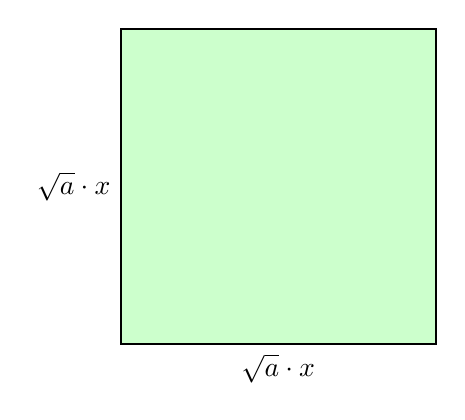
\begin{tikzpicture}[thick, scale=1]
        \fill [color=green,opacity=0.2] (0,0) rectangle +(4,4);
        \draw (0,0) rectangle +(4,4);
        \path (0,0) -- (4,0) node[midway,below] {$\sqrt{a}\cdot x$};
        \path (0,0) -- (0,4) node[midway,left] {$\sqrt{a}\cdot x$};
    \end{tikzpicture}
\end{center}

那么我们应该如何表示 $bx$ 这一项呢?我们要把正方形扩展到更大的正方形;这就是配方的意义。因此,我们需要围绕正方形构建一些矩形,这将有助于我们实现这一目标。让我们将 $bx$ 项代表的面积分成两个矩形,每个矩形的面积为 $\frac{b}{2}x$。由于矩形必须有一条边的长度为 $\sqrt{a} \cdot x$,并且我们希望矩形面积为 $\frac{b}{2}x$,因此另一条边长必然为 $\frac{b}{2\sqrt{a}}$: 

\begin{center}
    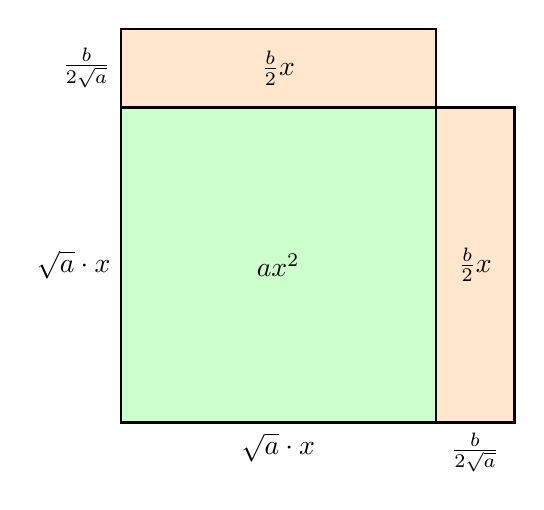
\begin{tikzpicture}[thick, scale=1]
        \fill [color=green,opacity=0.2] (0,0) rectangle +(4,4);
        \draw (0,0) rectangle +(4,4) node[pos=.5, align=center]{$ax^2$};
        \path (0,0) -- (4,0) node[midway,below] {$\sqrt{a}\cdot x$};
        \path (0,0) -- (0,4) node[midway,left] {$\sqrt{a}\cdot x$};

        \fill [color=orange,opacity=0.2] (4,0) rectangle +(1,4);
        \draw (4,0) rectangle +(1,4) node[pos=.5, align=center]{$\frac{b}{2}x$};
        \path (4,0) -- (5,0) node[midway,below] {$\frac{b}{2\sqrt{a}}$};

        \fill [color=orange,opacity=0.2] (0,4) rectangle +(4,1);
        \draw (0,4) rectangle +(4,1) node[pos=.5, align=center]{$\frac{b}{2}x$};
        \path (0,4) -- (0,5) node[midway,left] {$\frac{b}{2\sqrt{a}}$};
    \end{tikzpicture}
\end{center}

我们需要添加什么才能使上面的图形变成为一个正方形?我们发现只需在右上角填充一个小正方形即可。小正方形边长为 $\frac{b}{2\sqrt{a}}$,因此它的面积 --- 我们需要添加的项--- 为 $\frac{b^2}{4a}$。

\begin{center}
    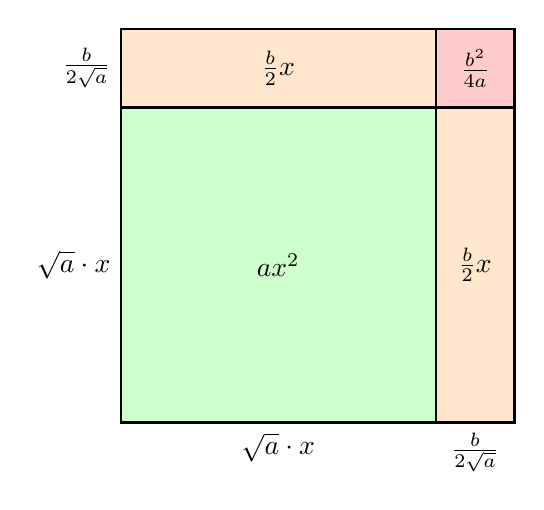
\begin{tikzpicture}[thick, scale=1]
        \fill [color=green,opacity=0.2] (0,0) rectangle +(4,4);
        \draw (0,0) rectangle +(4,4) node[pos=.5, align=center]{$ax^2$};
        \path (0,0) -- (4,0) node[midway,below] {$\sqrt{a}\cdot x$};
        \path (0,0) -- (0,4) node[midway,left] {$\sqrt{a}\cdot x$};

        \fill [color=orange,opacity=0.2] (4,0) rectangle +(1,4);
        \draw (4,0) rectangle +(1,4) node[pos=.5, align=center]{$\frac{b}{2}x$};
        \path (4,0) -- (5,0) node[midway,below] {$\frac{b}{2\sqrt{a}}$};

        \fill [color=orange,opacity=0.2] (0,4) rectangle +(4,1);
        \draw (0,4) rectangle +(4,1) node[pos=.5, align=center]{$\frac{b}{2}x$};
        \path (0,4) -- (0,5) node[midway,left] {$\frac{b}{2\sqrt{a}}$};

        \fill [color=red,opacity=0.2] (4,4) rectangle +(1,1);
        \draw (4,4) rectangle +(1,1) node[pos=.5, align=center]{$\frac{b^2}{4a}$};
    \end{tikzpicture}
\end{center}

看呐!这与我们上面通过代数推导得出的项完全相同。通过添加它,我们可以将这些项分解为完全平方。只需要再将其也减去,以确保原表达式不变。

这是一个需要记住的有用技巧。它可以提醒你配方的过程动机以及如何实现它。不过,你应该思考一件事:为什么这种可视化表示有效?我们必须假设 $a, b > 0$ 才能画出这些图,那么为什么无论 $a$ 和 $b$ 是什么,通向公式都有效呢?

\subsubsection*{二次函数求根公式}

让我们回到求多项式的根的问题。具体来说,让我们回忆一下\textbf{二次函数求根公式}。你可能已经记住这个公式是``求解二次方程''的一种方法,但你知道它为什么有效吗?让我们试着弄清楚吧!一般来说,我们从以下形式的二次多项式开始
\[p(x) = ax^2 + bx + c\]
其中 $a \ne 0$(否则,它就不是二次多项式),并且我们想要求 $p(x) = 0$ 时 $x$ 的值。(你是否尝试过回答我们上面提出的关于此类多项式有几个根的问题?在以下推导过程中请记住这些概念。)将该多项式因式分解为线性因子很麻烦,所以我们使用上面介绍的方法:配方。该方法的好处是,我们可以设置 $p(x)=0$,并在配方后重新整理项来求解 $x$。观察:
\[0 = p(x) = ax^2 + bx + c =a\Big(x+\frac{b}{2a}\Big)^2+\Big(c- \frac{b^2}{4a}\Big)\]
化简可得
\[\frac{b^2}{4a} -c = a\Big(x+\frac{b}{2a}\Big)^2\]

现在,我们要开始``撤消''此处的配方来求解 $x$,这需要对两边求平方根。但如果 $\frac{b^2}{4a} -c < 0$ 呢?我们根本无法求平方根!如果 $\frac{b^2}{4a} -c = 0$ 呢?会有问题吗?当 $\frac{b^2}{4a} -c > 0$ 时会有什么问题吗?这些问题与我们之前关于多项式可能有的根数相关。你可能已经(正确地)推断出二次多项式最多可以有两个根,但在这里我们发现二次多项式可能有一个或零个根(及其原因)!

\begin{itemize}
    \item 当 $\frac{b^2}{4a} -c < 0$ 时,那么 $x$ 的任何值都\emph{不}可能满足上面推导中的最后一行公式。因此,$p(x)$ 无实数根。
    \item 当 $\frac{b^2}{4a} -c = 0$ 时,那么对上面最后一行公式两边取平方根是完全有效的,但只会产生\emph{唯一一个 }$x$ 值:
    \begin{align*}
        \frac{b^2}{4a} -c = 0 &= a\Big(x+\frac{b}{2a}\Big)^2 \\
        0 &= x+\frac{b}{2a} \\
        x &= -\frac{b}{2a}
    \end{align*}
    \item 当 $\frac{b^2}{4a} -c > 0$ 时,此时,我们预期 $p(x)$ 有\emph{两个}根,因为两边取平方根会引入两个可能的解。一般来说,当我们遇到像 $s^2 = t$ 这种情况时,我们可以说唯一可能的解是 $s =\sqrt{t}$ 和 $s = -\sqrt{t}$,但我们必须同时考虑两者(通常将其写做 $s = \pm\sqrt{t}$)。在这种情况下求解 $x$ 得
    \begin{align*}
        \frac{b^2}{4a} -c &= a\Big(x+\frac{b}{2a}\Big)^2 \\
        \pm\sqrt{\frac{b^2-4ac}{4a}} &= \sqrt{a}\Big(x+\frac{b}{2a}\Big) = \sqrt{a}x+\frac{b}{2\sqrt{a}} \\
        -\frac{b}{2\sqrt{a}}\pm\frac{\sqrt{b^2-4ac}}{\sqrt{4a}} &= \sqrt{a}x \\
        -\frac{b}{2a}\pm\frac{\sqrt{b^2-4ac}}{\sqrt{4a^2}} &= x
    \end{align*}
    现在,我们必须小心对待之前进行的平方根观察。一般来说,$\sqrt{4a^2} = \pm2a$,但我们知道分子上的平方根项已经有一个相关的 $\pm1$ 因子,因此分母上的因子不会改变这一点。因此,我们可以得出结论
    \[x = -\frac{b}{2a}\pm\frac{\sqrt{b^2-4ac}}{2a} = \frac{-b\pm\sqrt{b^2-4ac}}{2a}\]
    这就是二次函数求根公式!
\end{itemize}

请记住,推导的最后一种情况是在 $\frac{b^2}{4a} -c > 0$ 的假设下进行的。当 $\frac{b^2}{4a} -c = 0$ 时,该公式依然适用吗?在这种假设下,我们是否可以执行与上面相同的步骤?为什么可以或者为什么不可以?

\subsubsection*{问题}

\begin{problem}
    找出 $a$ 的所有可能值,使 $x-a$ 是 $x^2+2ax-3$ 的因子。
\end{problem}
\begin{problem}
    找出 $b$ 的所有可能值,使得 $x^3 + b$ 可以被 $x + b$ 整除,没有余数。
\end{problem}
\begin{problem}
    对于任意自然数 $n$,因子 $x^n - 1$。
\end{problem}
\begin{problem}
    确定如下公式定义的 $x$ 的值
    \[x = \sqrt{2+\sqrt{2+\sqrt{2+\sqrt{2+\dots}}}}\]
    \begin{hint}
        尝试用 $x$ 本身来表示无限嵌套的平方根。
    \end{hint}
\end{problem}
\begin{problem}
    用配方法证明正数 $n$ 及其倒数之和始终大于或等于 $2$,并且唯一使和等于 $2$ 的数字是 $n = 1$。
    \begin{hint}
        求和,加减 $2$,然后重新整理。
    \end{hint}
\end{problem}
\begin{problem}
    如何求 $ax^4 + bx^2 + c$ 形式的四次多项式的根?
\end{problem}

\subsection{集合漫谈}

我们已经提到了一些特定类型的数字,但我们想具体定义我们将来要使用的数字集。这些数字集合都由一个特定字母用黑板粗体表示。\textbf{自然数}(也称为整体数(whole numbers)或计数数(counting numbers))之所以被称为自然数,是因为当我们计数物体时,用自然数感觉很``自然''。自然数可以写做
\[\mathbb{N} = \{1, 2, 3, 4, 5, \dots\}\]
(自然数有一个更具体更技术性的定义,我们将在稍后解释。)\\
我们用 $\mathbb{N}$ 表示 ``自然(natural)''

使用 $\mathbb{N}$,我们可以定义一个相关的数字集合:所有\textbf{整数}的集合,它包含了自然数、$0$ 和负自然数。整数可以写做
\[\mathbb{Z} = \{\dots, -3, -2, -1, 0, 1, 2, 3, \dots\}\]
字母 $\mathbb{Z}$ 来自德语单词 \emph{Zahlen},意思是``数字''。

从整数集合,我们可以定义\textbf{有理数}的集合。这些数字可以表示为整数的比率,但它们似乎没有像集合 $\mathbb{N}$ 和 $\mathbb{Z}$ 那样自然的``列表'',所以我们不能像上面那样书写这个集合。为此,我们使用一个非常常见的集合表示法,如下所示:
\[\mathbb{Q} = \Big\{\frac{a}{b} \mid a,b \in \mathbb{Z} \text{ 且 } b \ne 0\Big\}\]
读作:
\begin{quote}
    ``有理数集是所有 $\frac{a}{b}$ 形式的数的集合,其中 $a$ 和 $b$ 都是整数,且 $b$ 不为零。''
\end{quote}
这表达了有理数是分数的必要信息,其中分子和分母都是整数(但分母不能为 $0$,因为除以 $0$ 是不允许的)。我们使用字母 $\mathbb{Q}$ 表示有理数,是因为 $\mathbb{R}$ 已经被用于表示实数,而 $\mathbb{Q}$ 是上一个可用的字母。此外,$\mathbb{Q}$ 包含所有整数的商,所以这也是有道理的!

\textbf{实数} $\mathbb{R}$ 有一个非常技术性的定义,遗憾的是,我们无法在本书中全面深入研究。(这恰恰表明,从数学上定义这个集合是多么困难!) 目前,思考实数的一种方法是通过\textbf{数轴}。实数是数轴上所有的数字,而 $\mathbb{N}$、$\mathbb{Z}$ 和 $\mathbb{Q}$ 中的数字是数轴上的特定数字,它们并不构成整条数轴。某种程度上,$\mathbb{R}$ 是 $\mathbb{Q}$ 的``补全'',即``填补有理数之间的空白''。

\subsection{符号加油站}\label{sec:section1.3.5}

一种流行且方便的求和与求积的写法是使用缩写符号,将多个项或因子写成一种通用的形式。例如,如果我们想谈论前 $500$ 个自然数之和,该怎么写呢?写出总和的全部 $500$ 项会很乏味,所以 $1+2+3+\dots+499+500$ 是更常见的写法。(事实上,我们已经使用过这样的省略号。 你明白我们的意思吗?)这种写法很流行,并且确实表达了观点,但一些数学家对中间多余的省略号感到不满。我们推迟到现在才讨论这个问题,是因为符号通常很难学习和理解。我们并没有立即用新符号轰炸你,而是诉诸我们对 ``$\dots$'' 作用的直观理解。

既然我们已经提出来了,让我们看看如何避免使用省略号。为了写出我们上面提到的求和,我们将使用以下符号:
\[1+2+3+\dots+499+500 = \sum_{i=1}^{500}i\]
大写西格玛 $\sum$ 来自对应英文字母 S 的希腊字母,代表``求和''。\textbf{索引} $i$ 告诉我们求和的各个项的值。在 $\sum$ 符号下面写 $i = 1$,在 $\sum$ 符号上面写 $500$ 意味着我们让 $i$ 表示 $1$ 到 $500$(含)之间的所有自然数值。我们将这些值代入求和项的通用表达式,在本例中就是 $i$。因此,根据要求,求和项为 $1,2,3,\dots,500$。通过改变求和项表达式和/或索引的值,试着找到一些其他的写法。如果我们想求前 $500$ 个偶自然数之和怎么办?想求 $500$ 以内(含)所有偶自然数又该怎么办呢?尝试用上面的符号样式写出这些求和。

与此相关的是 $\prod$ 表示法。如果我们想查看前 $500$ 个自然数的乘积,我们将遵循相同的约定来识别索引值和通项:
\[1+2+3+\dots+499+500 = \prod_{i=1}^{500}i\]
大写派 $\prod$ 来自对应英文字母 P 的希腊字母,代表``求积''。再次尝试通过更改求积项和/或索引值以不同的方式表达上面公式。如果我们想求前 $500$ 个偶自然数的乘积怎么办?想求 $500$ 以内(含)所有偶自然数之积又该怎么办呢?尝试用上面的符号样式写出这些求积。

\subsubsection*{问题}

\begin{problem}
    用自然语言来描述以下等式的含义:
    \[\sum_{i=1}^{n}i^2 = \frac{n(n+1)(2n+1)}{6}\]
\end{problem}
\begin{problem}
    用适当的符号表达 $2$ 的前 $n$ 次幂的和与积,从 $2^0=1$ 开始。你能证明这个求和和求积公式吗?
\end{problem}
\begin{problem}
    考虑 $17$ 到 $33$(含)之间的所有奇数之和。索引 $0$ 开始,用求和符号写出这个求和公式。现在试着将索引从 $1$ 开始,重写求和公式。现在试着将索引从 $8$ 开始,重写求和公式,然后将索引从 $9$ 开始。以下哪一个感觉``更自然''?为什么?
\end{problem}
